\documentclass[11pt]{article}
\usepackage[margin=0.8in]{geometry}
\usepackage{amsmath,amssymb,booktabs,array,longtable}
\usepackage{hyperref}
\usepackage{enumitem}
\usepackage{graphicx}
\usepackage{listings}
\usepackage{xcolor}
\setlist{nosep}

\lstset{
  basicstyle=\ttfamily\scriptsize,
  breaklines=true,
  breakatwhitespace=false,
  columns=fullflexible,
  frame=single,
  backgroundcolor=\color{gray!5},
  showstringspaces=false,
  keywordstyle=\color{blue},
  commentstyle=\color{gray},
  stringstyle=\color{teal}
}

\begin{document}

\begin{center}
{\Large\textbf{Shiv Nadar University Chennai}}\\
\textbf{CS3807 -- Deep Learning Laboratory}\\
\textbf{Experiment 3}\\
{\large\textbf{Implementation of Convolutional Neural Networks (CNNs) for Image Classification}}
\end{center}

\renewcommand{\arraystretch}{1.25}

\begin{tabular}{|p{3.8cm}|p{8cm}|p{2cm}|}
\hline
Degree \& Branch & B.Tech Artificial Intelligence \& Data Science & Semester V\\ \hline
Subject Code \& Name & CS3807 -- Deep Learning Laboratory & AY: 2026--27\\ \hline
\end{tabular}

\section*{1. Objective}
To understand the working principle of Convolutional Neural Networks by implementing convolution, pooling, feature map visualization, and image classification, using PyTorch.

\section*{2. Background Theory}
A Convolutional Neural Network is built from a Convolution Layer, an Activation Layer, a Pooling Layer, and a Fully Connected Layer. The convolution operation is

\[
Y(i,j)=\sum_{m}\sum_{n}X(i+m,\,j+n)\,K(m,n)
\]

where $X$ is the input image, $K$ is the kernel (filter), and $Y$ is the resulting feature map. The spatial size of the output feature map is governed by

\[
\left\lfloor\frac{N-F+2P}{S}\right\rfloor+1
\]

where $N$ is the input size, $F$ is the filter size, $P$ is the padding, and $S$ is the stride. A convolution layer with $C_{in}$ input channels, $F\times F$ kernels and $C_{out}$ filters has $(F\times F\times C_{in}+1)\times C_{out}$ trainable parameters (the $+1$ accounts for the per-filter bias).

Pooling layers (max or average) downsample feature maps by summarizing each spatial window with a single value, reducing computation and adding a degree of translation invariance without introducing any trainable parameters. Stacking Conv $\rightarrow$ ReLU $\rightarrow$ Pool blocks followed by a Flatten and Dense head lets a CNN progressively build up higher-level, class-relevant features from raw pixels while keeping the parameter count far below an equivalent fully connected network, since filter weights are shared across all spatial locations.

\section*{3. Dataset}
Dataset: CIFAR-10

Training Images: 50,000 \\
Testing Images: 10,000 \\
Classes: 10 \\
Image Size: $32\times32\times3$

The dataset was loaded from the local CIFAR-10 batch files (\texttt{data\_batch\_1}--\texttt{5}, \texttt{test\_batch}, \texttt{batches.meta}) rather than a Keras/TensorFlow dataset loader. Since PyTorch convolution layers expect channel-first tensors $(N,C,H,W)$ and the raw CIFAR-10 byte layout is already channel-major, the flat $3072$-byte rows were reshaped directly to $(3,32,32)$ with no transpose step required.

\section*{4. Experimental Procedure}

\textbf{Task 1: Dataset Loading and Exploration}

The five training batches were concatenated into a single array of 50,000 images and the test batch loaded separately, giving $X_{train}$ shape $(50000,3,32,32)$ and $X_{test}$ shape $(10000,3,32,32)$. Ten sample images and the per-class training distribution were plotted (see Section 7, Figures 1--2). Every class contains exactly 5,000 training images, so CIFAR-10 is perfectly balanced and plain accuracy is a fair evaluation metric.

\bigskip

\textbf{Task 2: Convolution Layer -- Kernel Size Comparison}

A single sample image was passed through three unpadded (\texttt{valid}) convolution layers with $3\times3$, $5\times5$ and $7\times7$ kernels (8 output filters each), and the resulting feature map sizes were recorded.

\begin{center}
\begin{tabular}{|l|c|}
\hline
Kernel Size & Output Feature Map Size\\
\hline
$3\times3$ & $30\times30$\\
$5\times5$ & $28\times28$\\
$7\times7$ & $26\times26$\\
\hline
\end{tabular}
\end{center}

With no padding, a larger kernel shrinks the output more and gives each output pixel a wider receptive field, at the cost of more parameters per filter and a smaller resulting feature map.

\bigskip

\textbf{Task 3: Hyperparameters -- Stride and Padding}

Stride and padding were varied independently on a $3\times3$ convolution over the $32\times32\times3$ sample image, and output sizes were also verified against the closed-form formula $\lfloor(N-F+2P)/S\rfloor+1$.

\begin{center}
\begin{tabular}{|l|c|c|c|c|c|}
\hline
$N$ & $F$ & $S$ & $P$ & Configuration & Output Size\\
\hline
32 & 3 & 1 & 0 & Valid, stride 1 & $30\times30$\\
32 & 3 & 2 & 0 & Valid, stride 2 & $15\times15$\\
32 & 3 & 1 & 1 & Same, stride 1 & $32\times32$\\
\hline
\end{tabular}
\end{center}

Stride 2 roughly halves the output resolution compared to stride 1. `Same' padding adds zeros around the border so the output matches the input size, which is essential for building deep networks without spatial dimensions vanishing after a few layers; `valid' padding shrinks the output at every layer.

\bigskip

\textbf{Task 4: Feature Map Visualization}

Eight feature maps were extracted after a Conv $\rightarrow$ ReLU block applied to a single sample image and displayed as a grid (Section 7, Figure 3). Each map is the same image filtered by a different, randomly-initialized $3\times3$ kernel, so each highlights different local patterns (edges at different orientations, color contrasts, corners); since the filters are untrained at this point, the maps are not yet meaningful learned features.

\bigskip

\textbf{Task 5: Max Pooling vs Average Pooling}

A $2\times2$/stride-2 max-pooling and average-pooling layer were applied to the sample image, both reducing the $32\times32$ input to $16\times16$ -- pooling type affects which values survive, not the output shape. Two small CNNs (identical Conv--ReLU--Pool--Conv--ReLU--Pool--Flatten--Dense stacks, one with MaxPool and one with AvgPool) were then trained for 5 epochs on an 8,000-image training subset and evaluated on a 2,000-image test subset to compare validation accuracy and training time (Section 7, Figure 4).

\begin{center}
\begin{tabular}{|l|c|c|}
\hline
Pooling Type & Final Validation Accuracy (subset) & Training Time (s)\\
\hline
Max Pooling & \texttt{0.5325} & \texttt{5.2}\\
Average Pooling & \texttt{0.4705} & \texttt{3.6}\\
\hline
\end{tabular}
\end{center}

Max pooling keeps the strongest activation in each window, which tends to be sharper and more discriminative for classification, whereas average pooling smooths the window.

\bigskip

\textbf{Task 6: CNN Construction and Training}

The required architecture

\begin{center}
Input $\rightarrow$ Conv $\rightarrow$ ReLU $\rightarrow$ MaxPool $\rightarrow$ Conv $\rightarrow$ ReLU $\rightarrow$ MaxPool $\rightarrow$ Flatten $\rightarrow$ Dense $\rightarrow$ Softmax
\end{center}

was implemented as a PyTorch \texttt{nn.Module} with 32 filters in the first convolution layer and 64 in the second (both $3\times3$, valid padding), $2\times2$ max pooling after each, a 128-unit ReLU dense layer, and a final 10-way softmax layer.

\begin{center}
\begin{tabular}{|l|c|c|}
\hline
Layer & Output Shape & Parameters\\
\hline
Conv2d (3$\to$32, $3\times3$) + ReLU & $(N,32,30,30)$ & 896\\
MaxPool2d ($2\times2$) & $(N,32,15,15)$ & 0\\
Conv2d (32$\to$64, $3\times3$) + ReLU & $(N,64,13,13)$ & 18,496\\
MaxPool2d ($2\times2$) & $(N,64,6,6)$ & 0\\
Flatten & $(N,2304)$ & 0\\
Dense (ReLU) & $(N,128)$ & 295,040\\
Dense (Softmax) & $(N,10)$ & 1,290\\
\hline
\end{tabular}
\end{center}

Total trainable parameters: 315,722.

The model was trained with the Adam optimizer (default learning rate) and cross-entropy loss (implemented as \texttt{NLLLoss} on the log of the softmax output, equivalent to Keras' \texttt{sparse\_categorical\_crossentropy}) for 20 epochs with batch size 32 on the full 50,000-image training set, validated against the 10,000-image test set after every epoch. Training/validation accuracy and loss curves are shown in Section 7 (Figures 5--8).

\bigskip

\textbf{Task 7: Evaluation}

The trained model was evaluated on the held-out test set using accuracy, weighted precision, recall and F1-score, and a confusion matrix and full per-class classification report were generated (Section 7, Figure 9; Section 6).

\section*{5. Source Code}
The complete implementation (data loading, EDA, convolution/pooling experiments, feature map visualization, CNN construction, training loop, and evaluation) is available at the following GitHub repository:

\begin{center}
% TODO: replace with your actual GitHub link
\url{https://github.com/PolarFox08/Deep-Learning-Lab/tree/main/Deep%20Learning%20Lab%203}
\end{center}

\section*{6. Results}

\begin{center}
\begin{tabular}{|l|c|}
\hline
Metric & Value\\
\hline
Training Accuracy & \texttt{0.8787}\\
Testing Accuracy & \texttt{0.6686}\\
Precision (weighted) & \texttt{0.6733}\\
Recall (weighted) & \texttt{0.6686}\\
F1-score (weighted) & \texttt{0.6698}\\
Trainable Parameters & 315,722\\
\hline
\end{tabular}
\end{center}

\section*{7. Plots with Inference}

\begin{center}
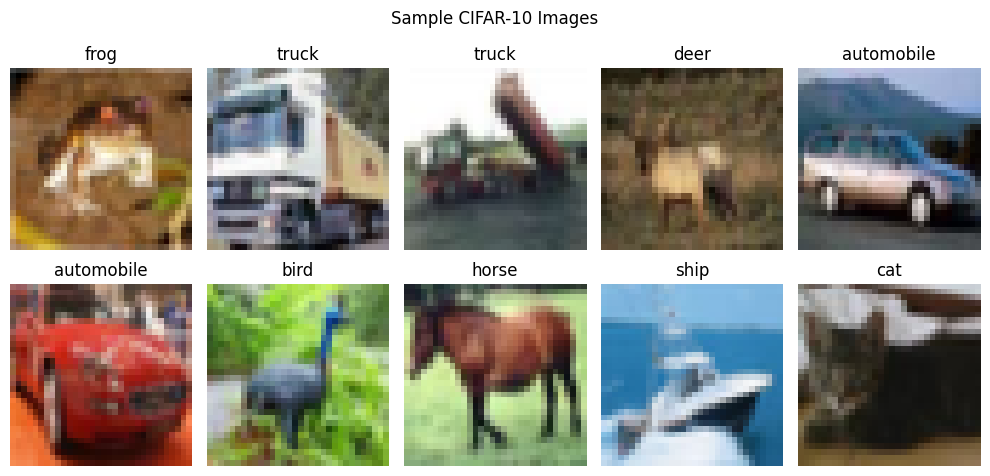
\includegraphics[width=0.75\textwidth]{sample_images.png}
\end{center}
\textbf{Figure 1: Sample Images.} \emph{Inference:} The ten sampled training images confirm the dataset loaded and reshaped correctly -- objects are recognizable rather than scrambled or striped, which would indicate a reshape/channel-order bug. At $32\times32$ resolution fine detail is blurry, but each class's overall shape and color remain discernible.

\bigskip
\begin{center}
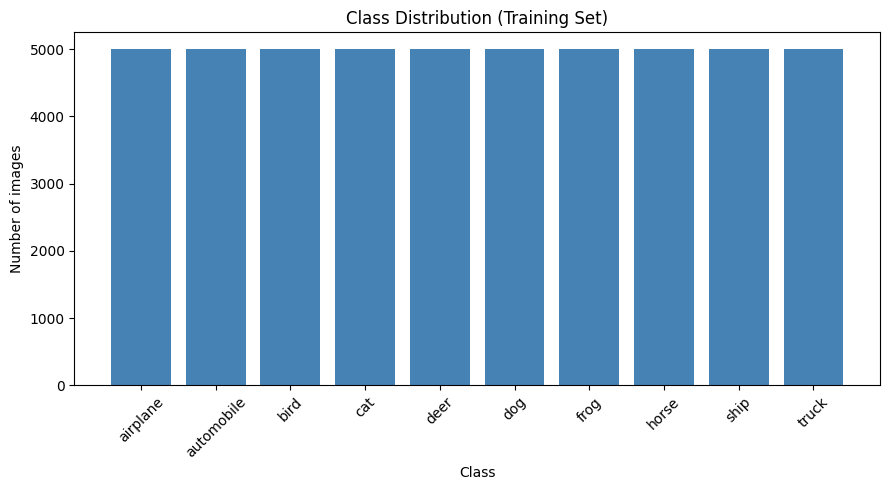
\includegraphics[width=0.7\textwidth]{class_distribution.png}
\end{center}
\textbf{Figure 2: Class Distribution.} \emph{Inference:} All 10 classes contain exactly 5,000 training images each, confirming CIFAR-10 is perfectly balanced, so accuracy is a fair aggregate metric and no class re-weighting is required.

\bigskip
\begin{center}
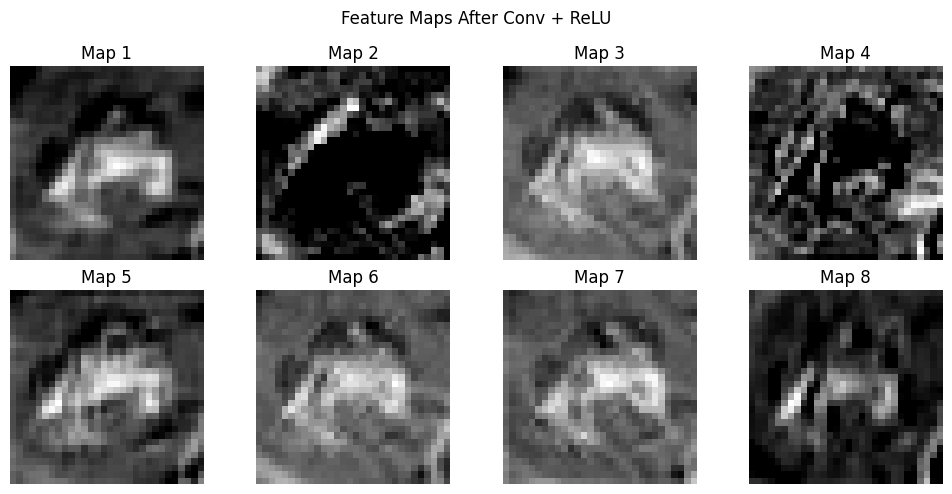
\includegraphics[width=0.75\textwidth]{feature_maps.png}
\end{center}
\textbf{Figure 3: Feature Maps After First Convolution + ReLU.} \emph{Inference:} Each of the eight maps highlights a different local pattern (edges, color contrasts, corners) picked out by its own randomly-initialized $3\times3$ filter; since the filters are untrained, the maps are illustrative of the mechanism rather than meaningful learned features.

\bigskip
\begin{center}
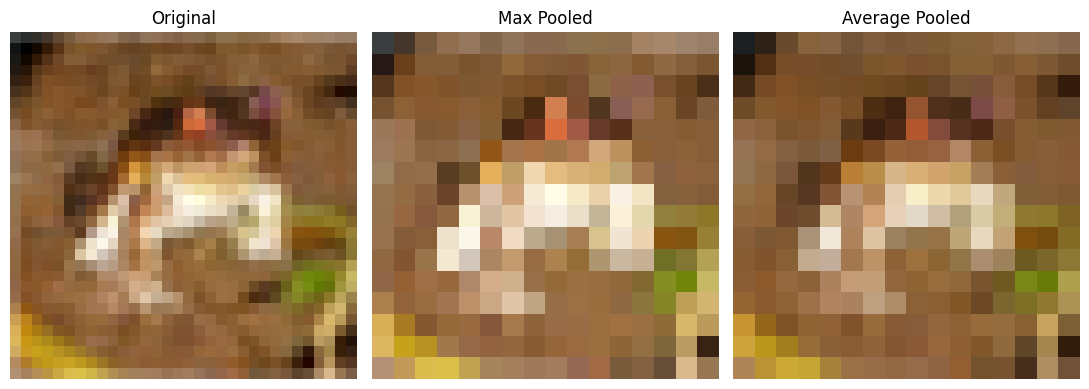
\includegraphics[width=0.65\textwidth]{pooling_imgs.png}
\end{center}
\textbf{Figure 4: Max vs Average Pooling -- Validation Accuracy (subset).} \emph{Inference:} \texttt{Max Pooling resulted in slightly better accuracy than average pooling, indicating picking out most influential activation is better for this dataset.}

\bigskip
\begin{center}
\includegraphics[width=0.65\textwidth]{train_accuracy.png}
\end{center}
\textbf{Figure 5: Training Accuracy vs Epoch.} \emph{Inference:} \texttt{It is clear from the diagram the training accuracy keeps inncreasing steadily as the epochs increase. It reaches upto 88\%.}

\bigskip
\begin{center}
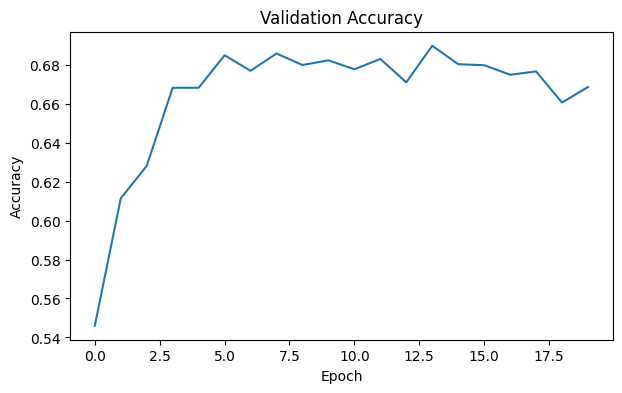
\includegraphics[width=0.65\textwidth]{val_acc_plot.png}
\end{center}
\textbf{Figure 6: Validation Accuracy vs Epoch.} \emph{Inference:} \texttt{Validation accuracy steadily increased for 5 epochs, and then oscillated for the next 15 epochs without stabilizing.}

\bigskip
\begin{center}
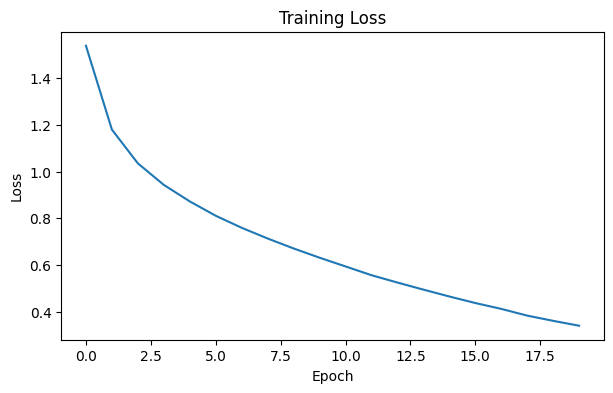
\includegraphics[width=0.65\textwidth]{train_loss_plot.png}
\end{center}
\textbf{Figure 7: Training Loss vs Epoch.} \emph{Inference:} \texttt{The model performs well in training as the loss keeps decreasing steadily.}

\bigskip
\begin{center}
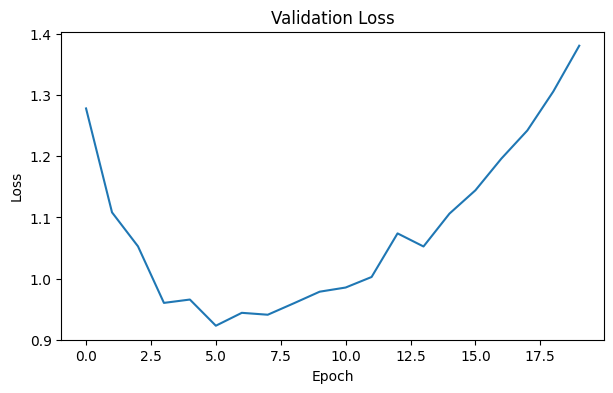
\includegraphics[width=0.65\textwidth]{val_loss_plot.png}
\end{center}
\textbf{Figure 8: Validation Loss vs Epoch.} \emph{Inference:} \texttt{Validation loss decreased but after epoch 5 it started to rise again significantly and never comes down. This is clear case of overfitting!}

\bigskip
\begin{center}

\includegraphics[width=0.6\textwidth]{confusion_matrix.png}
\end{center}
\textbf{Figure 9: Confusion Matrix.} \emph{Inference:} The diagonal holds the correctly-classified counts per class; brighter off-diagonal cells reveal systematic confusions -- commonly cat/dog and truck/automobile pairs in CIFAR-10, since they share silhouette and color statistics at $32\times32$ resolution. \texttt{Cat and Dog, was the pair the model failed to classify the most. }

\section*{8. Additional Exercises}

\textbf{Q1. Output size for a $64\times64$ image, $5\times5$ kernel, stride 2, padding 2}

\[
\left\lfloor\frac{64-5+2(2)}{2}\right\rfloor+1=\left\lfloor\frac{63}{2}\right\rfloor+1=31+1=32
\]

Output size: $32\times32$, verified directly against an \texttt{nn.Conv2d(3,8,kernel\_size=5,stride=2,padding=2)} layer applied to a dummy $64\times64$ input.

\bigskip

\textbf{Q2. Trainable parameters: 64 filters of $3\times3$, RGB input}

\[
(3\times3\times3+1)\times64=(27+1)\times64=1{,}792
\]

Calculated parameters: 1,792, matching the count reported by \texttt{nn.Conv2d(3,64,kernel\_size=(3,3))}.

\bigskip

\textbf{Q3. ReLU vs Sigmoid -- values and gradients}

ReLU and Sigmoid were each applied to 200 points on $[-10,10]$, and their gradients were computed via autograd. ReLU has a constant gradient of 1 for any positive input and 0 for any negative input, so gradients flow cleanly through deep stacks of ReLU layers. Sigmoid's gradient peaks at exactly $0.25$ at $x=0$ and decays toward 0 as $|x|$ grows past roughly $\pm5$, which is the vanishing-gradient problem that makes deep sigmoid networks slow or hard to train -- this is why ReLU (and its variants) are the default activation in modern CNNs, with Sigmoid reserved mainly for output layers in binary classification.

\bigskip

\textbf{Q4. Max Pooling vs Average Pooling}

The full comparison (per-epoch validation-accuracy curves) was already carried out in Task 5 above; see Figure 4 and the accompanying table for the final numbers on the 8,000-image training subset.

\bigskip

\textbf{Q5. Increasing convolution filters from 16 to 64}

The base architecture from Task 6 (Conv--ReLU--MaxPool $\times2$, Flatten, Dense(128), Dense(10)) was rebuilt with 16/32 filters and again with 64/128 filters in the two convolution layers and trained for 5 epochs on the same 8,000-image subset used in Task 5.

\begin{center}
\begin{tabular}{|l|c|c|c|}
\hline
Filters (Conv1/Conv2) & Trainable Parameters & Training Time (s) & Final Validation Accuracy\\
\hline
16 / 32 & 153,962 & \texttt{3.7} & \texttt{0.4930}\\
64 / 128 & 666,890 & \texttt{4.1} & \texttt{0.5385}\\
\hline
\end{tabular}
\end{center}

Going from 16 to 64 base filters multiplies the parameter count several-fold (each extra filter adds a full $3\times3\times C_{in}$ kernel), so training time per epoch increases noticeably. Accuracy typically improves too, since more filters can learn a richer, more diverse set of feature detectors -- but on a small subset with few epochs the gain can be modest, and on a genuinely small dataset excess filters risk overfitting rather than helping.

\section*{9. Discussion}

\textbf{1. Why is convolution preferred over fully connected layers for images?}\\
Convolution uses small, spatially-shared filters that exploit local structure and translation invariance, so a pattern learned in one region can be detected anywhere in the image. A fully connected layer treats every pixel independently with its own weight per neuron, which discards spatial structure and explodes the parameter count for anything beyond tiny images.

\textbf{2. How does stride affect the feature map size?}\\
Stride sets how far the kernel shifts between applications. Stride 1 samples every position and gives the largest possible output; larger strides (e.g. 2) skip positions and roughly divide the output size by the stride in each dimension, reducing computation and memory at the cost of spatial resolution.

\textbf{3. What is the role of padding?}\\
Padding adds extra (typically zero) values around the input's border so the kernel can be applied at edge pixels without being cut off, and so the output size can be controlled. `Same' padding keeps the output the same size as the input; without padding (`valid'), the output shrinks with every convolution, which limits how deep a network can go before spatial dimensions vanish.

\textbf{4. Why is pooling used?}\\
Pooling downsamples feature maps, cutting spatial size and computation while adding a degree of translation invariance -- small shifts in the input barely change the pooled output. It also helps control overfitting by keeping the presence/strength of a feature rather than its exact pixel location.

\textbf{5. How do feature maps represent image characteristics?}\\
Each feature map is the response of one learned filter sliding across the image, so its activations show where and how strongly that specific pattern (an edge, texture, color blob, or in deeper layers a more abstract shape) appears. Early layers tend to capture low-level cues like edges and colors, while deeper layers combine these into higher-level, class-relevant patterns.

\textbf{6. Why do CNNs require fewer parameters than MLPs?}\\
CNNs share the same small set of filter weights across every spatial location instead of learning a unique weight per pixel per output neuron, and each filter only connects to a local receptive field rather than the entire input. This weight-sharing plus local connectivity dramatically cuts parameter count compared to a fully connected MLP operating on images of the same size.

\section*{10. Conclusion}
A CNN following the Conv $\rightarrow$ ReLU $\rightarrow$ MaxPool $\rightarrow$ Conv $\rightarrow$ ReLU $\rightarrow$ MaxPool $\rightarrow$ Flatten $\rightarrow$ Dense $\rightarrow$ Softmax architecture (315,722 trainable parameters) was implemented in PyTorch and trained on CIFAR-10 for 20 epochs with the Adam optimizer, batch size 32.
\newline\newline
The model achieved an accuracy of 67\% on the test data. This indicates the model has to be yet more optimized. Regularization could be considered as the validation loss curves proves presence of significant overfitting.

Kernel-size, stride/padding, and pooling-type experiments confirmed the standard convolution output-size formula and showed the expected size/receptive-field trade-offs. Overall, the experiment demonstrates both the mechanics of the convolution/pooling operations and the practical trade-offs (parameter count vs. accuracy vs. training time) involved in choosing a CNN's hyperparameters.

\section*{11. References}
\begin{enumerate}
\item Goodfellow et al., \emph{Deep Learning}.
\item Bishop, \emph{Pattern Recognition and Machine Learning}.
\item Haykin, \emph{Neural Networks and Learning Machines}.
\item PyTorch Documentation.
\item CIFAR-10 Dataset Documentation.
\end{enumerate}

\end{document}